\documentclass[a4paper,11pt]{article}

\usepackage[utf8]{inputenc}
\title{ARC1 -- TP 7 et 8}
\author{Aurélien Anne, Léo Noël-Baron \& Thierry Sampaio}
\date{13/11/2015}


\usepackage{a4wide}
\usepackage{textcomp}
\usepackage[utf8]{inputenc}
\usepackage[T1]{fontenc}
\usepackage[francais]{babel}

\usepackage{graphicx}
\usepackage[usenames,dvipsnames]{color}

\usepackage{hyperref} \urlstyle{sf}
\hypersetup{
  colorlinks=true,
  urlcolor=BlueViolet,
  citecolor=BlueViolet,
  linkcolor=BlueViolet,
}
\DeclareUrlCommand\email{\urlstyle{sf}}

\newenvironment{keywords}
  {\description\item[\bsc{Mots-clés}]~$\cdot$~ }
  {\enddescription}
\newenvironment{remarque}
  {\description\item[\bsc{Remarque} ---]\sl}
  {\enddescription}
\renewcommand{\thefootnote}{\arabic{footnote}}

\usepackage{listings}
\lstset{
  language=C,
  basicstyle=\ttfamily,
  keywordstyle=\color{OliveGreen},
  stringstyle=\color{Bittersweet},
  showstringspaces=false,
  commentstyle=\color{Gray},
  numbers=left,
  numberstyle=\ttfamily\color{Gray},
  frame=l,
  columns=fullflexible,
  rulecolor=\color{Gray},
  tabsize=4,
  extendedchars=true,
  literate=
	{É}{{\'E}}1 {è}{{\`e}}1 {à}{{\`a}}1 {È}{{\`E}}1 {À}{{\`A}}1 {ê}{{\^e}}1 {â}{{\^a}}1 {î}{{\^\i}}1 {ô}{{\^o}}1
	{Ê}{{\^E}}1 {Â}{{\^A}}1 {Î}{{\^I}}1 {Ô}{{\^O}}1 {Û}{{\^U}}1 {ë}{{\"e}}1 {ï}{{\"\i}}1 {ü}{{\"u}}1 {Ë}{{\"E}}1
	{Ï}{{\"I}}1 {Ü}{{\"U}}1 {û}{{\^u}}1 {ç}{{\c c}}1 {Ç}{{\c C}}1 {æ}{{\ae}}1 {Æ}{{\AE}}1 {œ}{{\oe}}1 {Œ}{{\OE}}1
	{é}{{\'e}}1,
}
\lstMakeShortInline{|}

\parskip=0.3\baselineskip
\sloppy

\makeatletter
  \let\runtitle\@title
  \let\runauthor\@author
\makeatother

\usepackage{fancyhdr}
\pagestyle{fancy}
\fancyhead{}
\lhead{\runtitle}
\rhead{\runauthor}
\setlength{\headheight}{13.6pt}

\usepackage{amssymb}
\usepackage{tikz}

\setlength{\parindent}{0em}
\usepackage{array}

\begin{document}

\maketitle

\begin{abstract}
Ce TP vise à concevoir un circuit capable de maintenir le maximum, et le nombre d'occurrences de ce maximum, parmi une suite d'entiers entrés un à un.
\end{abstract}

\subsection*{Spécifications et algorithme}

Le circuit demandé intègre une commande d'initialisation, une opérande sur 4 bits pour l'entrée des nombres et une commande pour signaler au circuit de traiter l'entrée. Ses sorties sont le maximum courant et son nombre d'occurrences sur 4 bits, ainsi qu'un signal indiquant la validité des deux précédentes et la possibilité d'entrer un nouveau nombre.

Un tel circuit doit suivre l'algorithme suivant :
\begin{verbatim}
Si Init
    Max <- 0
    CptMax <- 0
    Prêt <- 1
Si Dem
    charger E[3..0]
    Si E > Max
        Max <- E
        CptMax <- 0
    Si E = Max
        CptMax <- CptMax + 1
\end{verbatim}

La relative complexité du sujet rend pertinente une conception selon le modèle UC/UT.

\subsection*{Unité de traitement}

D'après l'algorithme précédent, nous proposons une UT disposant des commandes suivantes :
\begin{itemize}
  \item initialiser les valeurs ;
  \item charger un nouveau nombre en vue de son traitement ;
  \item incrémenter le compteur d'occurrences du maximum ;
  \item mettre à jour le maximum avec le nombre chargé.
\end{itemize}

Notre UT comprendra donc une entrée de commande sur 2 bits, l'opérande de chargement sur 4 bits et en sortie le maximum actuel et son nombre d'occurrences, ainsi que deux signaux comparant le nombre chargé et le maximum actuel (selon les relation inférieur strict et supérieur strict). Ces deux derniers signaux permettront à l'UC de sélectionner les commandes à activer dans le bon ordre, selon le nombre entré.

Une réalisation possible d'une telle UT est donnée en Figure \ref{UT} ; le registre du haut contient le nombre chargé, celui de droite le maximum actuel et le compteur maintient le nombre d'occurrences. Les commandes de chargement des registres, d'incrémentation et de remise à zéro du compteur sont induites par la commande de l'UT. La réutilisation du composant SEL4 en bas à droite permet de gérer la remise à zéro du registre $Max$, et le composant COMP4 donne les signaux $inf$ et $sup$.

\begin{figure}[h]
\center
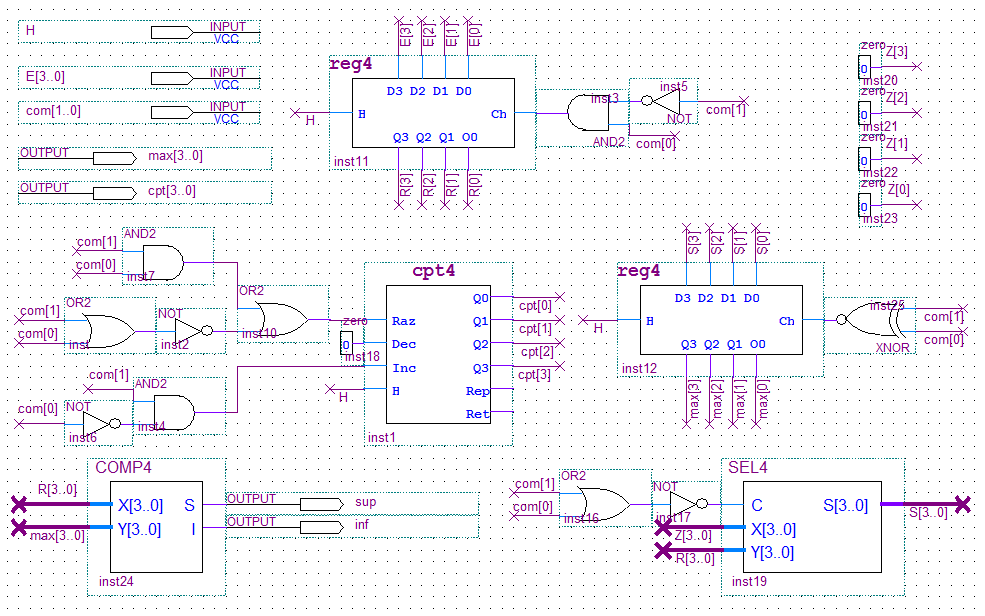
\includegraphics[scale=0.6]{UT.png}
\caption{Circuit de l'unité de traitement}
\label{UT}
\end{figure}

\subsection*{Unité de contrôle}

Le protocole demande/réponse imposé correspond à l'automate présenté en Figure \ref{autoUC}. L'initialisation se fait à l'état 0 ; l'état 1 attend l'entrée d'un nombre, avant de le charger dans l'état 2. Selon le cas, c'est ensuite l'état 3 qui met à jour le maximum et passe au 4, ou le 4 qui incrémente le compteur et passe au 5, ou directement le 5 qui attend la retombée de la demande avant de revenir à l'état 1.

\begin{figure}[h]
\center
\begin{tikzpicture}[scale=0.17]
\tikzstyle{every node}+=[inner sep=0pt]
\draw [black] (22.1,-46.5) circle (3);
\draw (22.1,-46.5) node {$0$};
\draw [black] (22.1,-30) circle (3);
\draw (22.1,-30) node {$1$};
\draw [black] (41.4,-30) circle (3);
\draw (41.4,-30) node {$2$};
\draw [black] (41.4,-13.7) circle (3);
\draw (41.4,-13.7) node {$3$};
\draw [black] (63,-30) circle (3);
\draw (63,-30) node {$4$};
\draw [black] (41.4,-46.5) circle (3);
\draw (41.4,-46.5) node {$5$};
\draw [black] (16.9,-46.5) -- (19.1,-46.5);
\draw (16.4,-46.5) node [left] {$Init$};
\fill [black] (19.1,-46.5) -- (18.3,-46) -- (18.3,-47);
\draw [black] (22.1,-43.5) -- (22.1,-33);
\fill [black] (22.1,-33) -- (21.6,-33.8) -- (22.6,-33.8);
\draw [black] (19.814,-28.075) arc (257.62938:-30.37062:2.25);
\draw (16.28,-22.28) node [right] {$\overline{Dem}$};
\fill [black] (22.24,-27.01) -- (22.9,-26.34) -- (21.92,-26.13);
\draw [black] (25.1,-30) -- (38.4,-30);
\fill [black] (38.4,-30) -- (37.6,-29.5) -- (37.6,-30.5);
\draw (31.75,-30.5) node [below] {$Dem$};
\draw [black] (41.4,-27) -- (41.4,-16.7);
\fill [black] (41.4,-16.7) -- (40.9,-17.5) -- (41.9,-17.5);
\draw (41.9,-21.85) node [right] {$sup$};
\draw [black] (43.79,-15.51) -- (60.61,-28.19);
\fill [black] (60.61,-28.19) -- (60.27,-27.31) -- (59.67,-28.11);
\draw [black] (44.4,-30) -- (60,-30);
\fill [black] (60,-30) -- (59.2,-29.5) -- (59.2,-30.5);
\draw (52.2,-30.5) node [below] {$\overline{sup}\cdot\overline{inf}$};
\draw [black] (60.62,-31.82) -- (43.78,-44.68);
\fill [black] (43.78,-44.68) -- (44.72,-44.59) -- (44.12,-43.8);
\draw [black] (41.4,-33) -- (41.4,-43.5);
\fill [black] (41.4,-43.5) -- (41.9,-42.7) -- (40.9,-42.7);
\draw (41.9,-38.25) node [right] {$inf$};
\draw [black] (42.723,-49.18) arc (54:-234:2.25);
\draw (41.4,-53.75) node [below] {$Dem$};
\fill [black] (40.08,-49.18) -- (39.2,-49.53) -- (40.01,-50.12);
\draw [black] (39.12,-44.55) -- (24.38,-31.95);
\fill [black] (24.38,-31.95) -- (24.66,-32.85) -- (25.31,-32.09);
\draw (37.46,-37.76) node [left] {$\overline{Dem}$};
\end{tikzpicture}
\caption{Diagramme des états de l'unité de contrôle}
\label{autoUC}
\end{figure}

On en déduit le circuit de la Figure \ref{UC} pour un codage à un bit par état ; la génération des commandes suit alors les formules $c_1=q_3+q_4$ et $c_0=q_1+q_2+q_3+q_5$, et le signal prêt doit être levé quand l'automate est dans l'état 1.

\begin{figure}[h]
\center
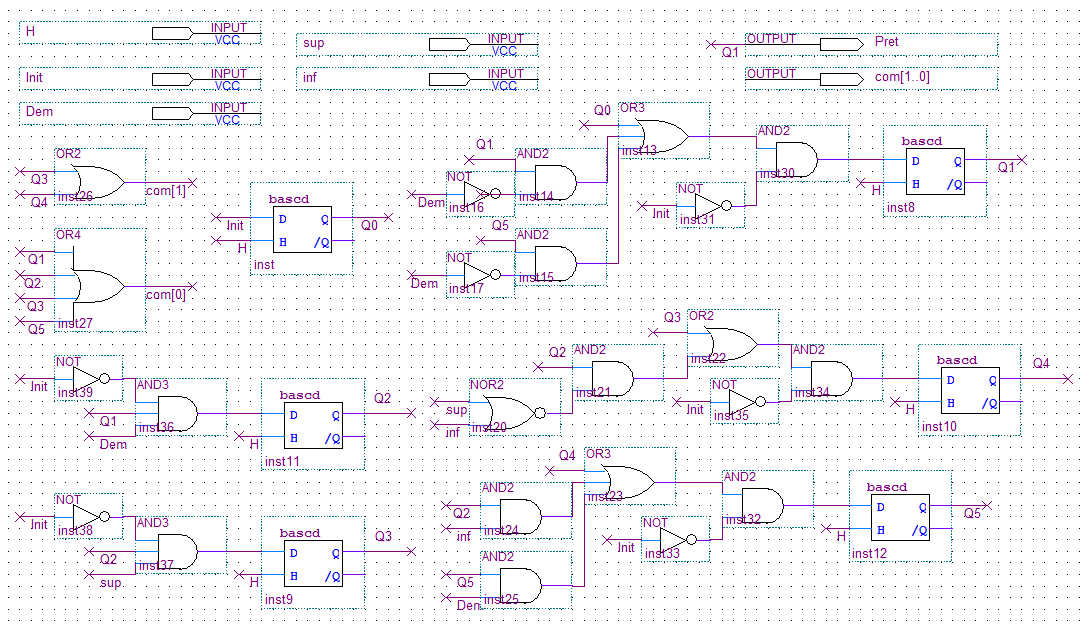
\includegraphics[scale=0.5]{UC.png}
\caption{Circuit de l'unité de contrôle}
\label{UC}
\end{figure}

\subsection*{Circuit complet}

Les branchements entre l'unité de contrôle et l'unité de traitement sont évidents et donnent le circuit présenté en Figure \ref{max}.

\begin{figure}[h]
\center
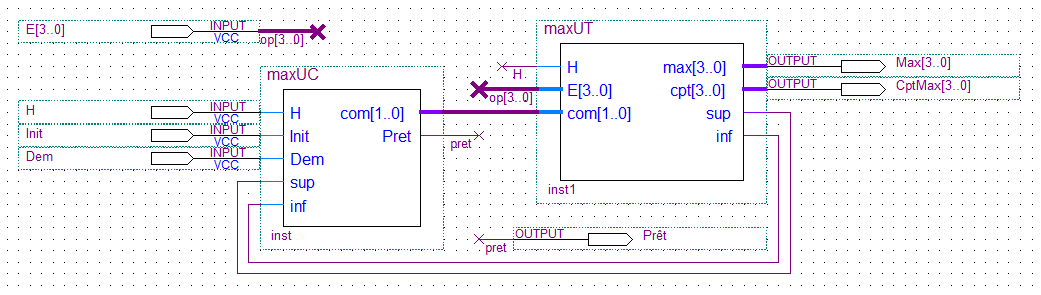
\includegraphics[scale=0.55]{MaxSeq.png}\vspace*{1em}
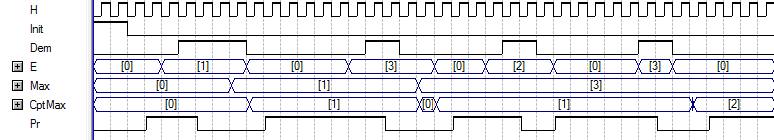
\includegraphics[scale=0.6]{sim.png}
\caption{Circuit final et simulation}
\label{max}
\end{figure}

\end{document}
